\section{Experimental Results}\label{sec:4experiment}
In this section, we first evaluate the performance of \systemname in detecting individual sleep-related events
(Sec.~\ref{sec:exp:individuals}). We then compare \systemname against alternative schemes for sleep stage detection
(Sec.~\ref{sec:overall_per}). Finally, we demonstrate the usefulness of \systemname in helping users to understand and improve their sleep
through user study (Sec.~\ref{sec:user_survey}).

\subsection{Evaluation of Event Detection\label{sec:exp:individuals}}
In this sub-section, we evaluate the accuracy of \systemname on detecting five sleep events: the body posture, the body rollover, the hand
position, micro-body movements and acoustic events. Unless otherwise stated, the ground truth of an event is obtained by watching or
listening to the video/audio footage.



\subsubsection{Sleep Posture Detection}
\label{subsub:bodyposture} Fig.~\ref{fig:posture_zhu} reports the sleep posture detection accuracy for individual users. \systemname
achieves a consistent detection accuracy of over 90\% across testing users and postures. The confusion matrix in Table \ref{tab:posture}
shows that \systemname only misclassifies a posture on a few occasions, leading to an overall detection precision of over 96\% across
users. This performance is better than the one reported by SleepMonitor~\cite{sleepmonitor}. In particular, {\systemname} gives an
improvement of 5\% for the prone state and has an overall lower false positive rate. Furthermore, {\systemname} is able to detect more hand
positions during sleeping when compared to SleepMonitor. In terms of errors, due to angular characteristics of acceleration being similar
between the supine posture where the hand is put on the head and the left-lateral posture, a small amount of the supine postures are
misclassified as the left lateral. From the results, we can also observe that the total number of detected prone postures is smaller than
that for other postures. This suggests that our testing users are not used to sleep in this position, because it is neither healthy nor
comfortable.






\begin{figure}
	\centering
	\begin{minipage}{.5\textwidth}
	 \centering
	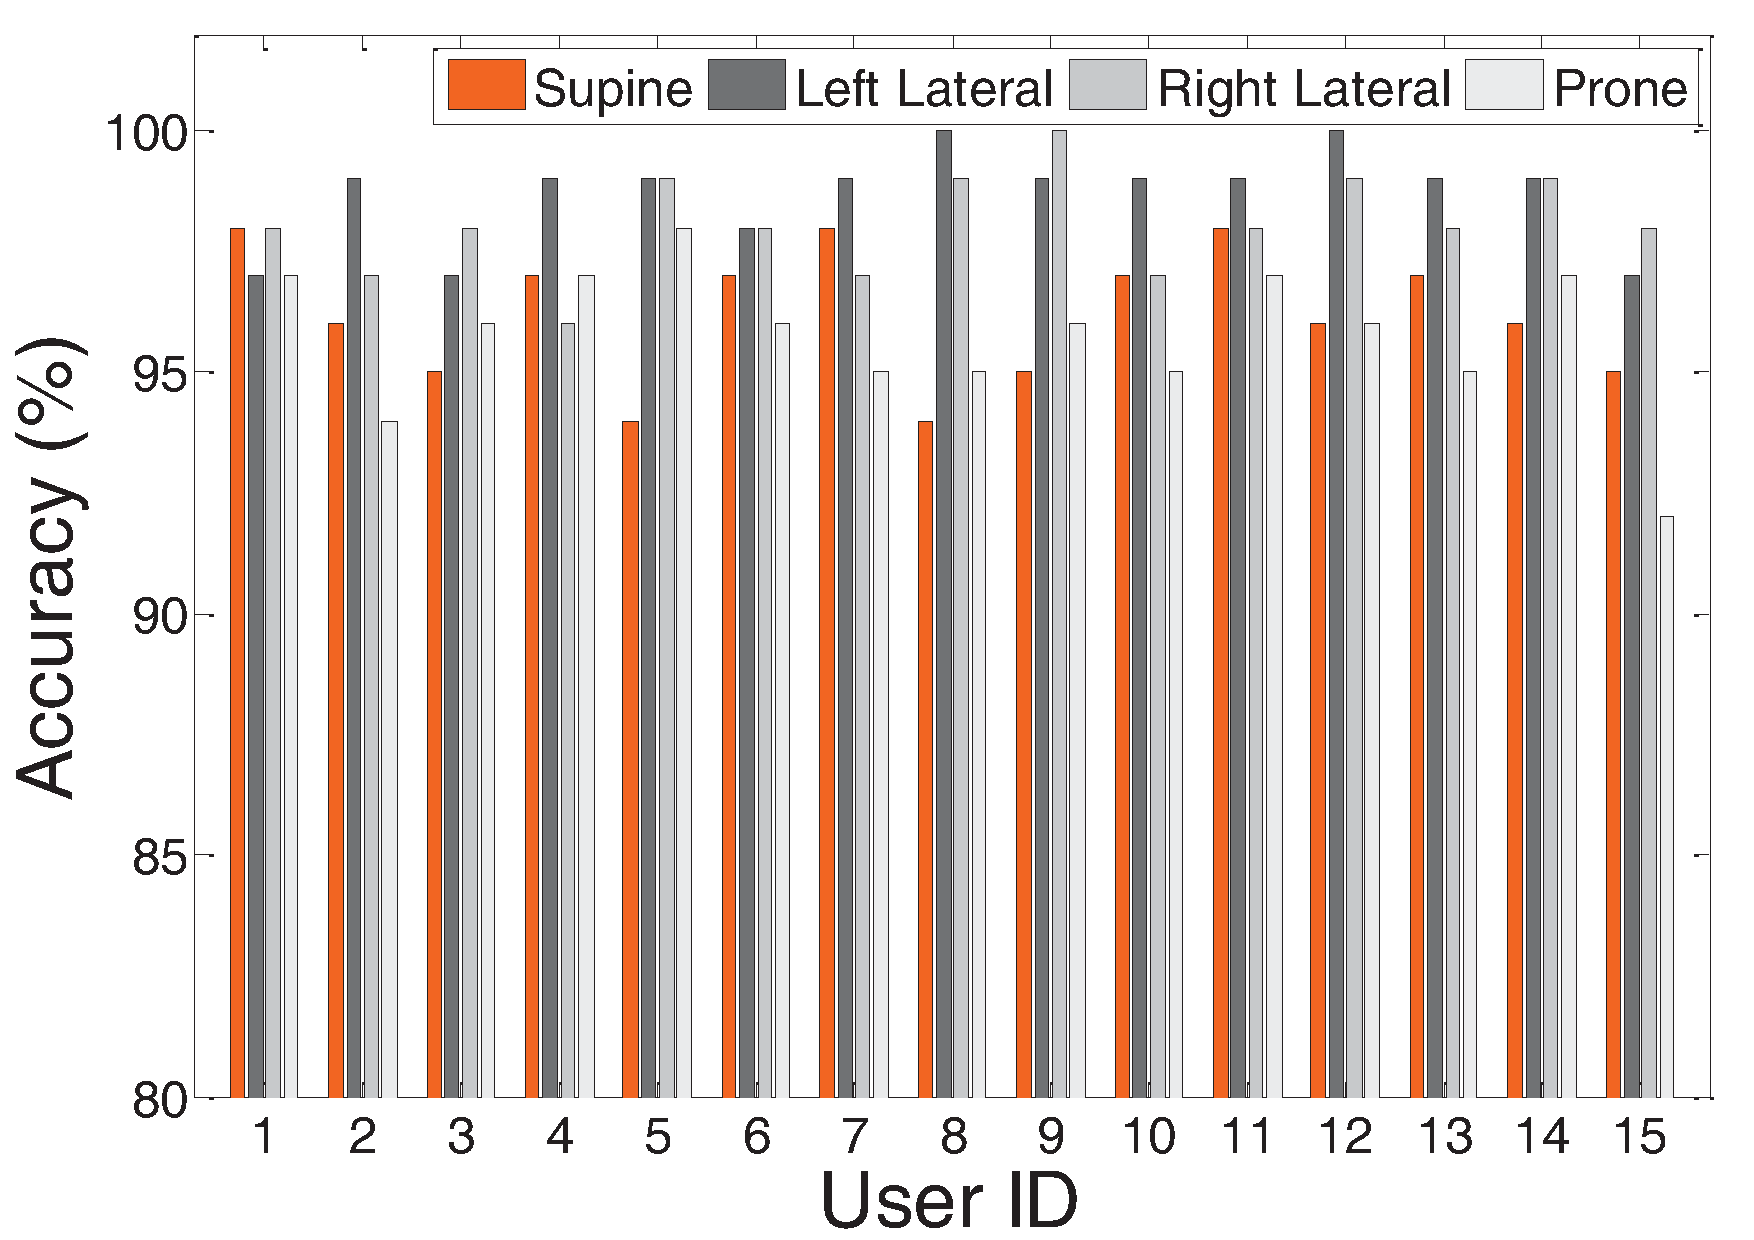
\includegraphics[width=0.95\linewidth]{Figures/posture_zhu.pdf}
	\caption{Detection accuracy of body postures.}\label{fig:posture_zhu}
	\end{minipage}%
	\begin{minipage}{.5\textwidth}
			\centering
		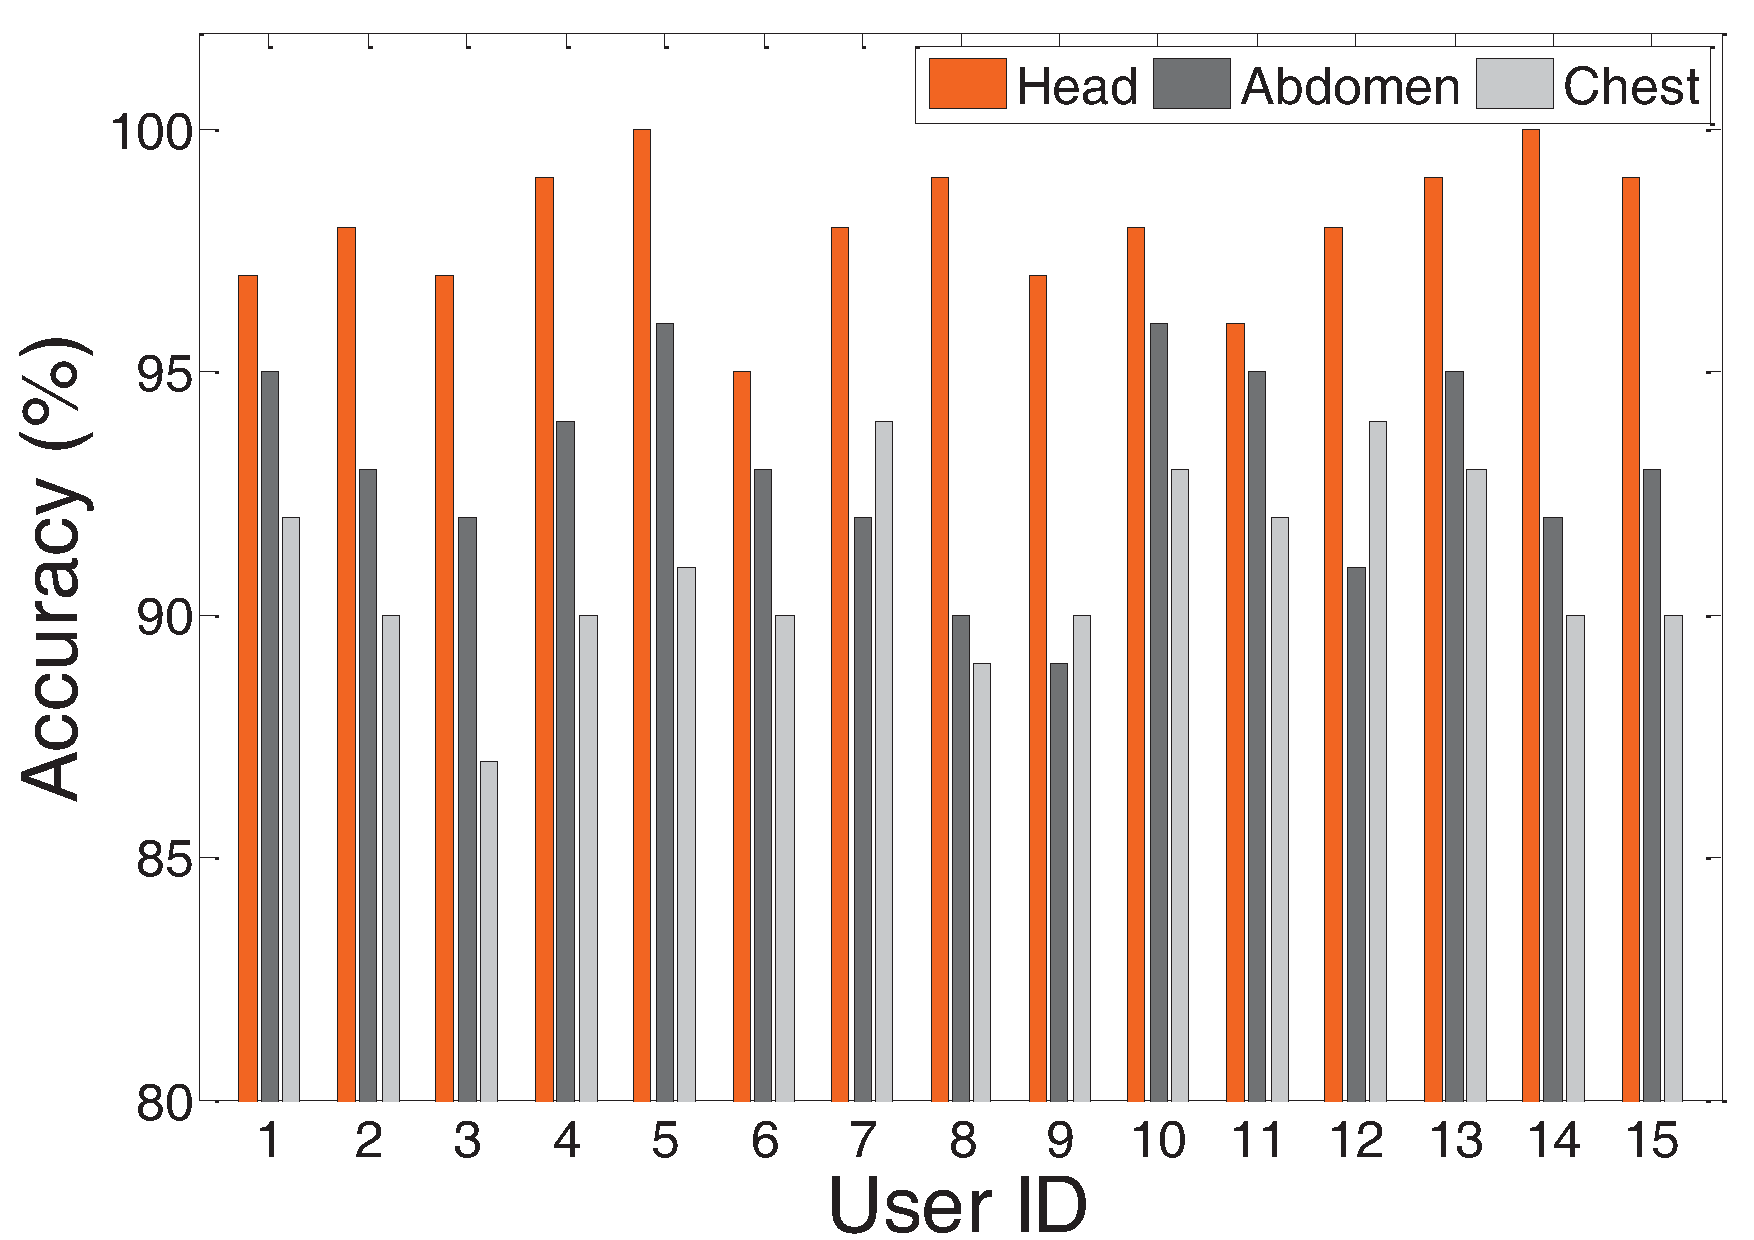
\includegraphics[width=0.95\linewidth]{Figures/handposition_zhu.pdf}
		\caption{Identification accuracy of hand positions.}\label{fig:hand_zhu}
	\end{minipage}
\end{figure}

\begin{table}[!t]\footnotesize
	\centering
	\renewcommand\arraystretch{0.35}
	\caption{The confusion matrix of body posture classification.}\label{tab:posture}
	\begin{tabular}{c| r | r | r | r | r | r}
		\cline{1-7}
		&\multicolumn{1}{ c|}{ }
		& \multicolumn{4}{ c|}{ }\\
		\multirow{2}*{}
		&\multicolumn{1}{c|}{\multirow{2}*{{\textbf{Result}}}}
		&\multicolumn{4}{c|}{{\textbf{Prediction}}}
		& \multirow{4}*{{\textbf{Recall}}} \\
		\cline{3-6}
		& & & & & \\
		\multicolumn{1}{c|}{{}}
		&  \multicolumn{1}{c|}{{}}
		&  \multicolumn{1}{l|}{{Supine}}
		&  \multicolumn{1}{l|}{{Left Lateral}}
		&  \multicolumn{1}{l|}{{Right Lateral}}
		&  \multicolumn{1}{l|}{{Prone}}   \\
		& & & & & \\
		\cline{1-7}
		& & & & & \\
		\multirow{5}{*}{\begin{sideways}{{Groundtruth}}\end{sideways}}
		&   {Supine}   & {\bf{{1182}}}    &   $25$      &   $4$      &   $9$    &   {96.7\%}\\
		& & & & & \\
		\cline{2-7}
		& & & & & \\
		&   {Left Lateral}   &   $6$      &   {\bf{{1292}}}     &   $0$      &   $0$   &   {99.5\%} \\
		& & & & & \\
		\cline{2-7}
		& & & & & \\
		&   {Right Lateral}   &   $7$      &   $0$      &  {\bf{{1275}}}      &   $12$  &   {98.5\%}  \\
		& & & & & \\
		\cline{2-7}
		& & & & & \\
		&   {Prone}   &   $19$      &   $2$      &   $3$      &   {\bf{{567}}}   &   {95.9\%} \\
		& & & & & \\
		\cline{1-7}
		& & & & & \\
		&   {Precision}    &   {97.3 \%}   &   {98.0\%}   &   {99.5\%}   &   {96.4\%}    \\
		& & & & & \\
		\cline{1-7}
	\end{tabular}
\end{table}


\subsubsection{Body Rollover Counting}
Table \ref{tab:rollver} reports the performance of body rollover counting. Three of our participants, users 3, 4 and 13, have an unusually
high number of rollovers. For users 3 and 4, they have difficulties in falling asleep due to the sleep disorder, while user 13 needs to
rollover frequently because of his loudly snoring. As we will demonstrate in Sec.~\ref{sec:user_survey}, these participants also suffered
from poor sleep quality and hence indicate how the information extracted by {\systemname} can support the detection of sleep problems. For
all the 15 users, the detection accuracies are all high with the lowest accuracy of 87\%. Therefore, {\systemname} can accurately
distinguish  large hand movements from body rollovers. We stress the the small detection errors in body rollover events do not have a
significant impact on our end result. This is because for sleep stage detection, we consider a multiple events in addition to body
rollover, including micro-body movement and acoustic events, which can offset the detection errors for body rollover.

\begin{table}[!t]\footnotesize
  \caption{Detection accuracy of body rollovers.}\label{tab:rollver}
  \setlength{\tabcolsep}{3pt}
\renewcommand{\arraystretch}{0.67}{\multirowsetup}{\centering}
        \begin{tabular}{lccccccccccccccc}
        \toprule
         \textbf{Testing User ID}    & 1& 2  & 3& 4& 5& 6& 7& 8& 9& 10& 11& 12& 13& 14& 15\\
        \midrule
            \rowcolor{Gray} {Labeled \#body-rollover}  &231&204&442&397&198&101&196&164&193&208&131&205&342&149&156 \\
                 {Accuracy} &91\%& 94\% &88\%&93\%&96\%&94\%&87\%&90\% &93\% &94\% &92\% &94\% &89\% &90\% &95\%\\
        \bottomrule
 \end{tabular}
\end{table}

\subsubsection{Hand Position Recognition}
Recall that we combine the tracked hand movement trajectory and periodic signals caused by respiration to identify if the hand is placed on
the chest, addomen or head. In our dataset, 14\%, 36\% and 22\% of the time the hand in the supine posture during sleep were placed on the
head, abdomen, and chest respectively. Fig.~\ref{fig:hand_zhu} illustrates the accuracy of hand position across 15 users. As we can see
that using just one single user's data for training, our approach achieves an accuracy of over 87\% across different testing users.
Moreover, we find that at least 4 out of our 15 participants tended to put their hands on their heads (which often lead to bad sleep) and
one participate unconsciously put his hand on the chest (which is likely to cause nightmares). By identifying these hand positions,
\systemname can inform users to change their sleeping behaviors.

\subsubsection{Micro-body Movement Detection}

In this experiment, in addition to manually labeling the ground truth from the video footage, we also use the accelerometer in the
smartphone placed on the bed to record the occurrence of micro-body movements - hand movements, arm raising and body trembling. Using the
smartphone data to obtain the ground truth prevents us from missing some movements such as trembling concealed by the duvet (which may not
be visible from the video). To gather ground truths from the smartphone data, we first smooth the collected acceleration data along the
three axes. Next, we calculate the Root Sum Square (RSS) value to merge the results across axes to obtain the first-order derivative of the
merged acceleration data (see Sec.~\ref{sec:microbo}). Then, we use the threshold-based method described in Sec.~\ref{sec:microbo} to mark
the occurrence of micro-body movements from the smartphone data. The marked smartphone data is then used together with the manually labeled
micro-body movements as the ground truths.

Table~\ref{tab:micro_move} lists the total number of the micro-body movements for each participant over the testing period of 14 days, and
Fig.~\ref{fig:micro_movement_zhu} reports the accuracy of {\systemname} for detecting these micro-body movements. As can be seen from the
table and figure, \systemname delivers consistently good precision across our testing users. Figure~\ref{fig:micro_combine} reports the
averaged accuracy across users. The averaged accuracies for arm raising and body trembling are higher, 93\% and 84\% respectively. While we
achieve the lowest accuracy for detecting hand movements, the average procession and recall still exceed 78\%. The accuracy for detecting
hand movements and body trembling can be further improved by using more training data collected from a longer period of time. It is to note
that the purpose of micro-body movement detection is to detect different sleep stages. Since hand movements usually appear in all sleep
stages, they offer little information gain for identifying sleep stages compared to other micro-body movements.  As a result, the
relatively low detection accuracy of hand movements has little impact on sleep stage detection.


\begin{figure*}
	\centering
	\begin{minipage}{.485\textwidth}
		 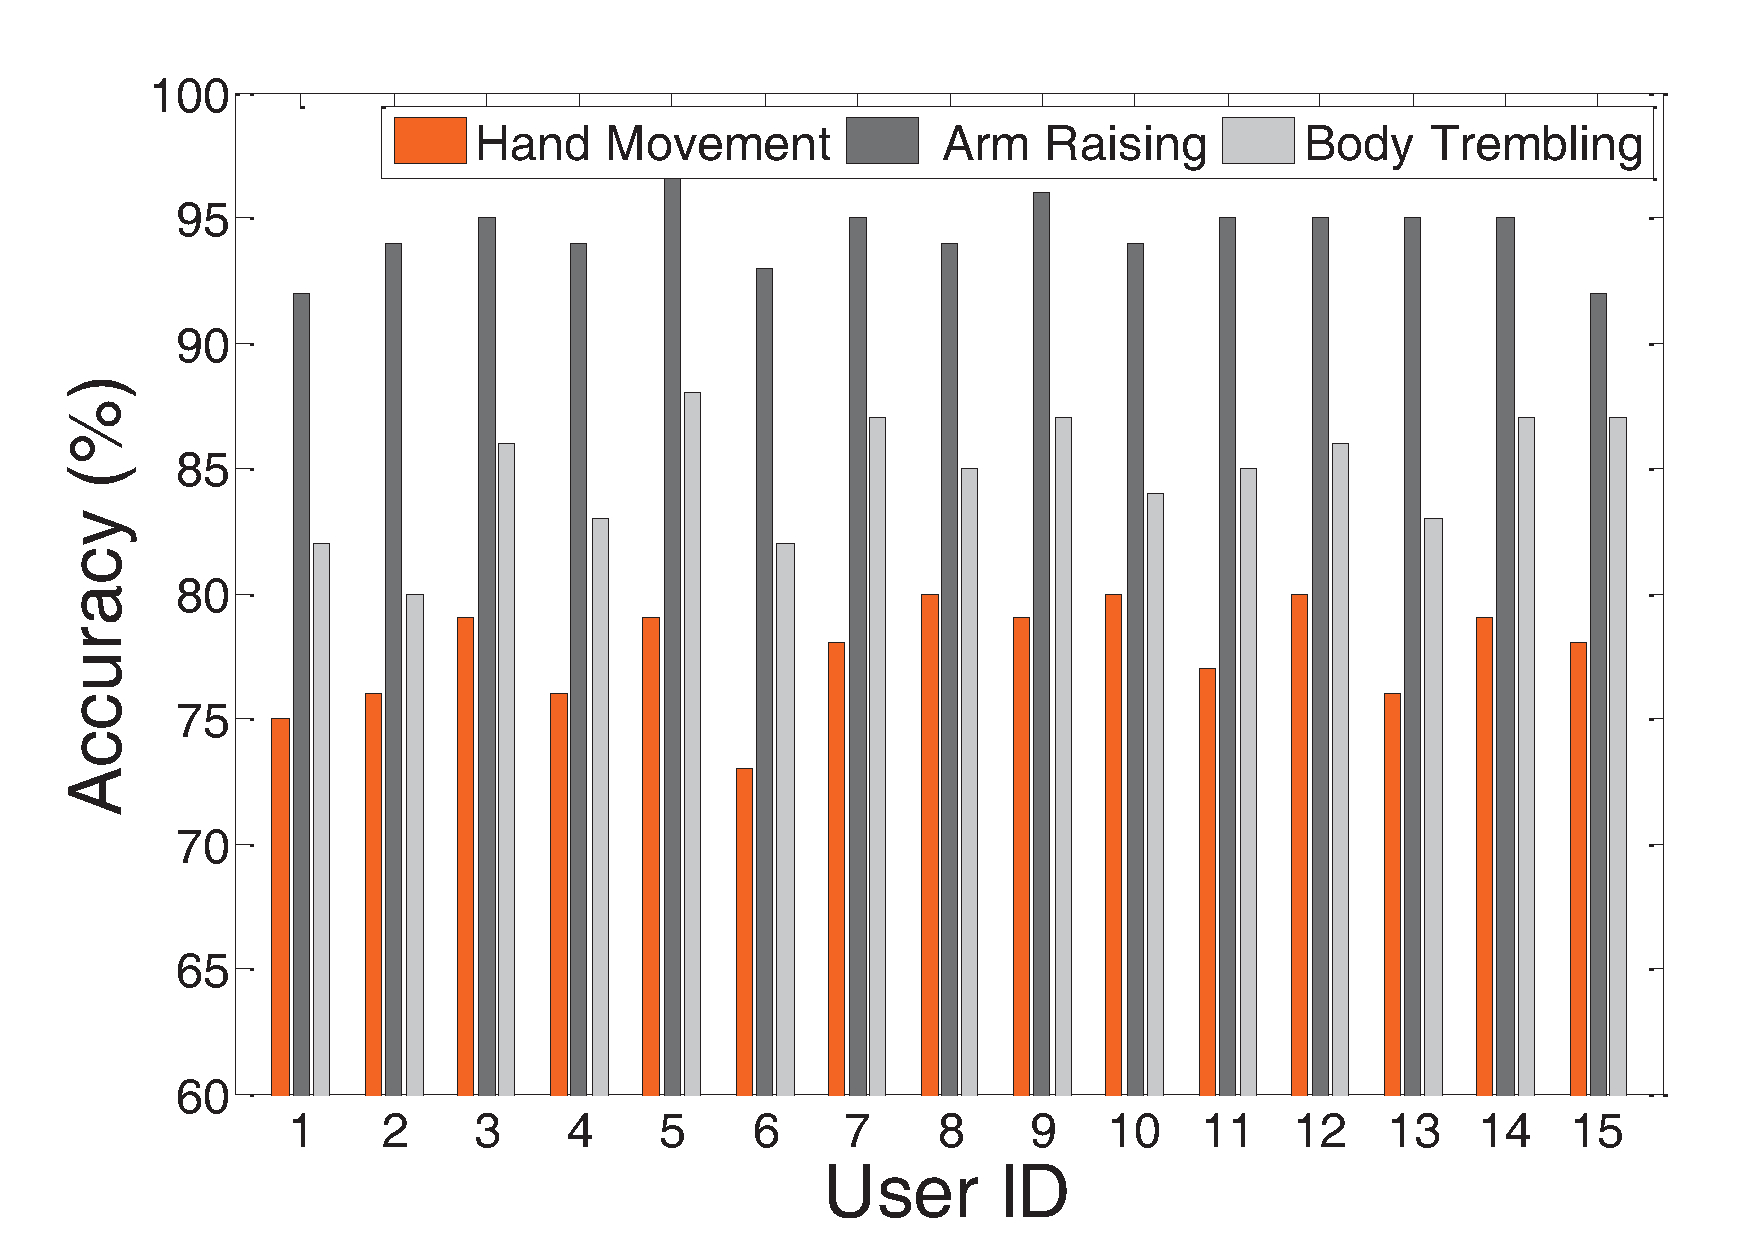
\includegraphics[width=0.95\textwidth]{Figures/micro_movement_zhu.pdf}
		\caption{Micro-body movement detection for each user.}\label{fig:micro_movement_zhu}	
	\end{minipage}%
\hspace{3pt}
	\begin{minipage}{.485\textwidth}
	 \centering
	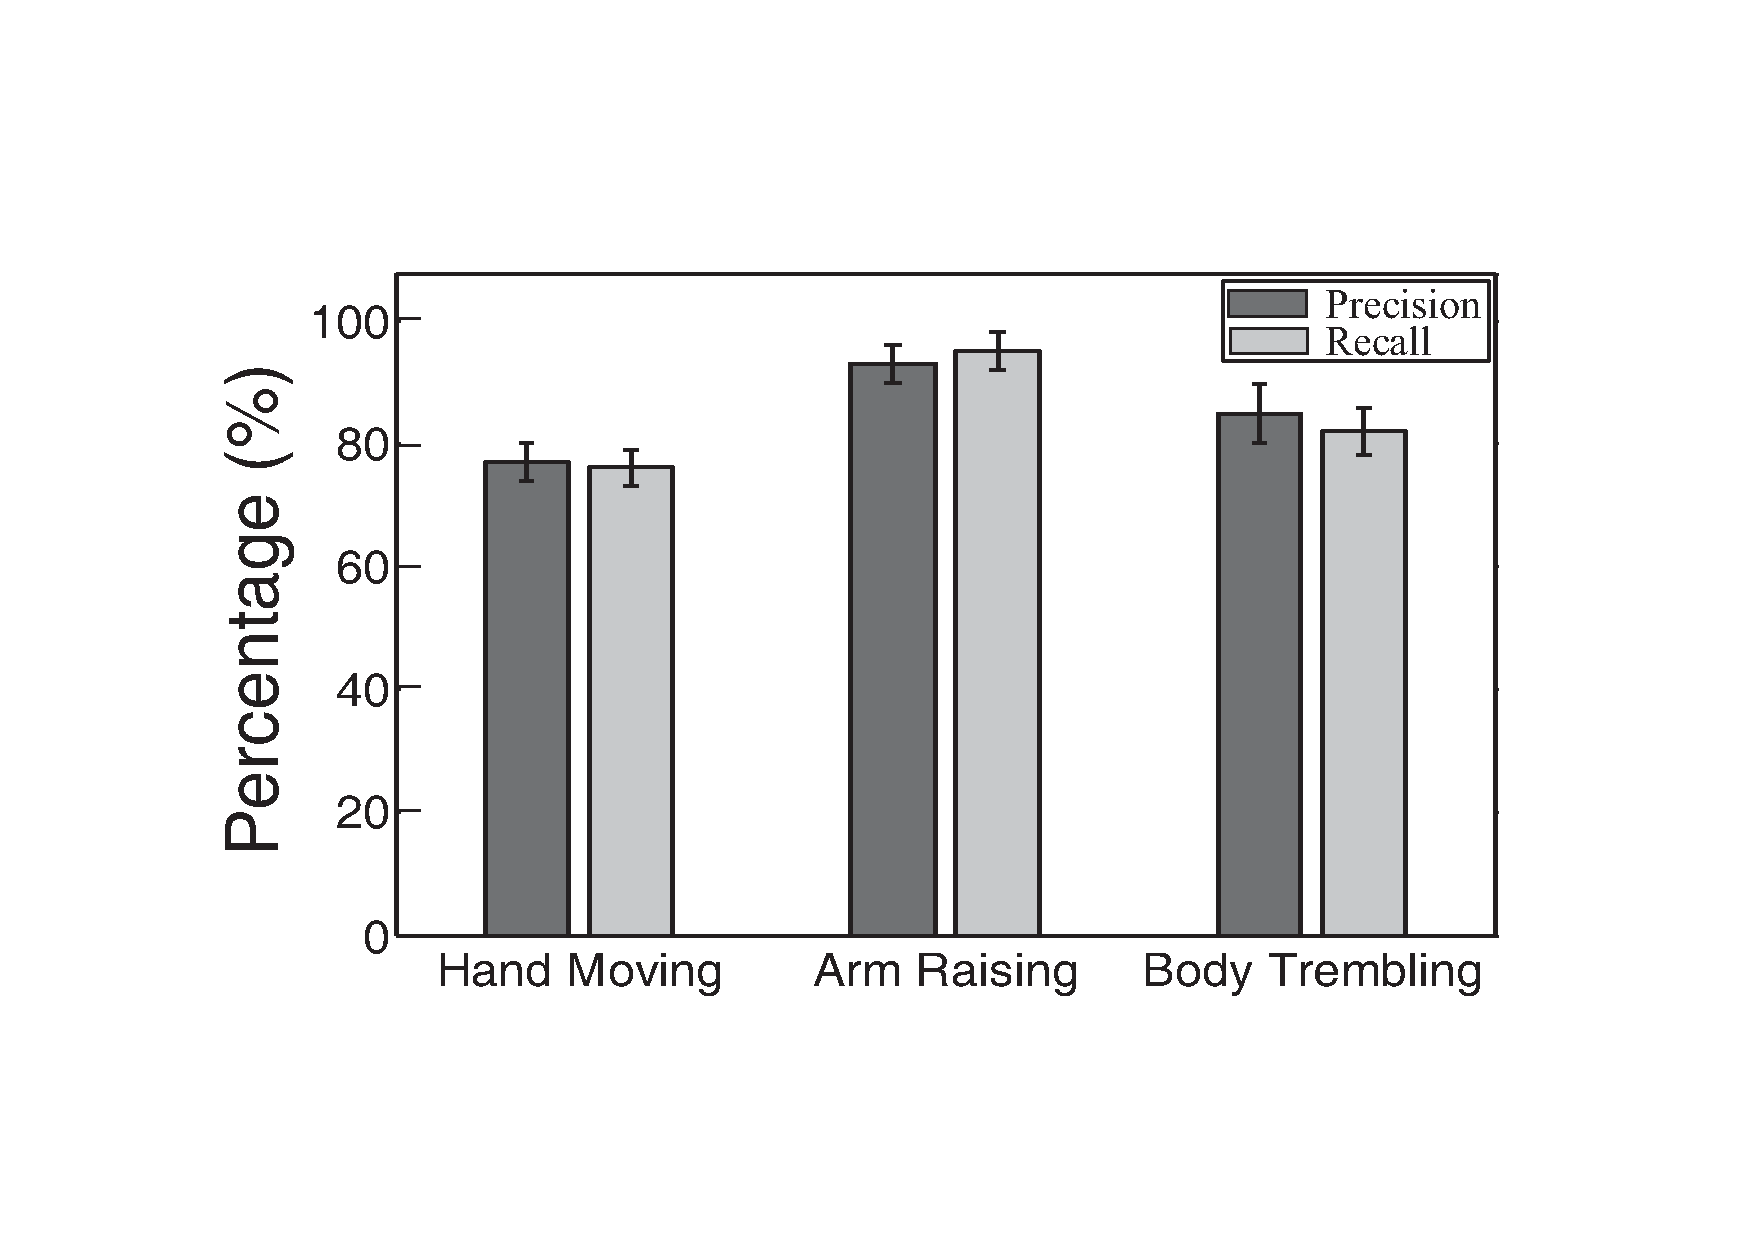
\includegraphics[width=7.8cm,height=5cm]{Figures/micro_combine1.pdf}
	\caption{Average precision and recall for micro-body movement detection.}\label{fig:micro_combine}
	\end{minipage}
\end{figure*}


\begin{table}[!t]\footnotesize
  \caption{The number of micro-body movements per user.}\label{tab:micro_move}
   \renewcommand\arraystretch{1}{\multirowsetup}{\centering}
        \begin{tabular}{lccccccccccccccc}
        \toprule
         \textbf{Testing User ID}    & 1& 2  & 3& 4& 5& 6& 7& 8& 9& 10& 11& 12& 13& 14& 15\\
        \midrule
            \rowcolor{Gray} {Labeled \#hand movement}  &52&49&67&55&78&65&59&70&61&53&81&55&60&59&63 \\
             { Labeled \#arm raising} &48&50&62&53&66&49&57&50&73&45&54&69&57&56&61\\
             \rowcolor{Gray} { Labeled \#body trembling} &28&32&25&29&34&25&20&30&24&26&27&35&24&22&25\\
        \bottomrule
 \end{tabular}
\end{table}


 \subsubsection{Acoustic Events Detection}
 Table~\ref{tab:sound} shows the results for acoustic event detection across 15 participants. Overall, \systemname is highly accurate in
 detecting acoustic events, with an average accuracy of over 88\%. The precision for detecting coughs is
88.9\%, which is slightly lower than for the other three event types. The reason is that different users have distinct cough patterns but
the pre-defined parameters in the detection model do not include all patterns. For examples, some people have a fast and continuous pattern
of coughing, while others have a slower intermittent pattern. Our model for cough detection is trained on 120 sets of nighttime sound data
collected from users who are different from our testing users. To further improve accuracy, we can either specialize our model using data
collected from the target user or using a larger and more diverse set of training data. Nonetheless, \systemname is able to detect acoustic
events with a high accuracy.


\begin{table}[!t]\footnotesize
  \centering
 \renewcommand\arraystretch{0.35}
  \caption{The confusion matrix of acoustic events detection.}\label{tab:sound}
   \vspace{-2mm}
\begin{tabular}{c| r | r | r | r | r | r}
   \hline
   &\multicolumn{1}{ c|}{ }
   & \multicolumn{4}{ c|}{ }\\
   \multirow{2}*{}
&\multicolumn{1}{c|}{\multirow{2}*{{ \textbf{Result}}}}
&\multicolumn{4}{c|}{{ \textbf{Prediction}}}
& \multirow{4}*{{ \textbf{Recall}}} \\
    \cline{3-6}
    & & & & & \\
    \multicolumn{1}{c|}{{}}
    &  \multicolumn{1}{c|}{{}}
    &  \multicolumn{1}{l|}{{ Snore}}
    &  \multicolumn{1}{l|}{{ Cough}}
    &  \multicolumn{1}{l|}{{ Somniloquy}}
    &  \multicolumn{1}{l|}{{ Other}}   \\
    & & & & & \\
     \cline{1-7}
    & & & & & \\
    \multirow{5}{*}{\begin{sideways}{{ Ground truth}}\end{sideways}}
    &   { Snore}   & {\bf{{96}}}    &   $0$      &   $0$      &   $9$    &   {91.4\%}\\
    & & & & & \\
    \cline{2-7}
    & & & & & \\
   &   { Cough}   &   $3$      &   {\bf{{64}}}     &   $0$      &   $4$   &   {90.1\%} \\
    & & & & & \\
     \cline{2-7}
    & & & & & \\
    &   { Somniloquy}   &   $0$      &   $3$      &  {\bf{{42}}}      &   $2$  &   {89.4\%}  \\
    & & & & & \\
     \cline{2-7}
    & & & & & \\
    &   { Other}   &   $0$      &   $5$      &   $4$      &   {\bf{{325}}}   &   {97.3\%} \\
    & & & & & \\
    \hline
    & & & & & \\
    &   { Precision}      &   {96.9\%}   &   {88.9\%}   &   {91.3\%}   &   {95.6\%}    \\
    & & & & & \\
    \hline
   \end{tabular}
\end{table}


\subsection{Evaluation of Sleep Stage Detection\label{sec:overall_per}}
In order to prove that \systemname is able to identify the sleep stages but not just user's sleep habits, we use the results given by
Fitbit Charge2 as the ground truth. In this evaluation, we randomly choose a total of $50$ sets  of sleep data for 15 participants across
two weeks, yielding at least $3$ sets per participant.

{\systemname} uses event-driven methods to  detect changes in the sleep stage. To identify sleep stages, \systemname uses sleep events
detected within a 15-minute window. The window starts from the first detected event. If no event was detected within 15 minutes, it assumes
the sleep stage remains unchanged.

\subsubsection{Sleep Stage Detection}
\begin{table}[!t]\footnotesize
%\setlength{\tabcolsep}{1pt}
\renewcommand{\arraystretch}{0.55}{\centering}
	\caption{{The confusion matrix of sleep stage detection.}}\label{tab:sleep stage}
 \vspace{-2mm}
	\begin{tabular}{c| r | r | r | r | r}
		\hline
		&\multicolumn{1}{ c|}{ }
		& \multicolumn{3}{ c|}{ }\\
		\multirow{2}*{}
		&\multicolumn{1}{c|}{\multirow{2}*{{ \textbf{Result}}}}
		&\multicolumn{3}{c|}{{ \textbf{Prediction}}}
		& \multirow{3}*{{ \textbf{Recall}}} \\
		%&\multicolumn{5}{ c |}{\textbf{\small Prediction}} \\
		% & \multicolumn{5}{ c |}{ } \\
		\cline{3-5}
		& & & & & \\
		\multicolumn{1}{c|}{{}}
		&  \multicolumn{1}{c|}{{}}
		&  \multicolumn{1}{l|}{{ REM}}
		&  \multicolumn{1}{l|}{{ Light Sleep}}
		&  \multicolumn{1}{l|}{{ Deep Sleep}} \\
		\cline{1-6}
		& & & & & \\
		\multirow{1}{*}{\begin{sideways}{{Ground truth}}\end{sideways}}
		&   { REM}   & {\bf{{476}}}    &   $143$      &   $61$     &   {70.0\%}\\
		& & & & & \\
		\cline{2-6}
		& & & & & \\
		&   { Light Sleep}   &   $131$      &   {\bf{{508}}}     &   $91$      &   {69.6\%} \\
		& & & & & \\
		\cline{2-6}
		& & & & & \\
		&   { Deep Sleep}   &   $63$      &   $113$      &  {\bf{{262}}}      &   {59.8\%}  \\
		& & & & & \\
		\cline{1-6}
		& & & & & \\
		&   { Precision}      &   {71.0\%}   &   {66.5\%}   &   {63.3\%}   \\
		& & & & & \\
		\hline
	\end{tabular}
\end{table}

%In this specific experiment, we use \emph{cross-validation} to train and evaluate our algorithms. Specifically, we train our algorithms
%using the data collected from one participant and apply the learned algorithms to the remaining 14 participants. We repeat this process by
%using each participant's data as the training data in turn. We then report the the average performance across the cross-validation folds.
%This is a standard evaluation methodology, providing an estimate of the generalization ability of a predictive model when processing
%\emph{unseen} data. The reason of training our algorithms on a single-user is to evaluate if \systemname can obtain accurate results using
%a small set of training data.


The averaged precision and recall for sleep stage detection are given in Table~\ref{tab:sleep stage}. Overall, \systemname is able to
correctly identify over 60\% of the sleep stages. While {\systemname} can mis-predict between the light sleep and the REM stages, the
overall performance is not far from FitBit. Moreover, as we will demonstrate later, the main benefits of {\systemname} are its capability
to capture a wide range of sleep events and how do they correlate to sleep quality, but not for accurate sleep stage detection (where
medical PSG measurements will be required).



\subsubsection{Impact of Respiratory Amplitudes on Sleep Stage Detection}

When detecting different sleep stages, \systemname also considers the respiratory amplitude when the hand is put on the abdomen or chest.
To assess the effectiveness of respiratory amplitude estimation, we evaluate the performance of the sleep stage detection with and without
taking the respiration amplitude into account. The performance of sleep stage detection is shown in Table~\ref{tab:respiratory}. For the
three different sleep stages, both precision and recall are improved between 5\% to 10\% with the help of respiratory amplitude estimation.
An alternative to our approach is to use the respiratory frequency  as a feature for sleep stage detection. We found that this alternative
scheme gives similar performance for sleep stage detection as our approach. This is because the respiratory amplitude is strongly
correlated with the respiratory frequency -- when the respiratory amplitude is larger, the time taken for one breath will be longer, and
consequently the frequency of breathing will be slower.

\begin{table}[!t]\footnotesize
	\centering
	\renewcommand\arraystretch{0.3}
	\caption{Effect of respiratory amplitude estimation.}\label{tab:respiratory}
 \vspace{-2mm}
	\begin{tabular}{l| l | r | r | r | r | r | r |}
		\cline{2-8}
		&\multicolumn{1}{ c|}{ }
		&\multicolumn{2}{ c|}{ }
		&\multicolumn{2}{ c|}{ }
		& \multicolumn{2}{ c|}{ }\\
		%  \multirow{4}*{}
		&\multicolumn{1}{c|}{}
		&\multicolumn{2}{c|}{\textbf{\footnotesize REM}}
		&\multicolumn{2}{c|}{\textbf{\footnotesize Light Sleep}}
		&\multicolumn{2}{c|}{\textbf{\footnotesize Deep Sleep}} \\
		%&\multicolumn{5}{ c |}{\textbf{\small Prediction}} \\
		% & \multicolumn{5}{ c |}{ } \\
		\cline{2-8}
		& & & & & & &\\
		\multicolumn{1}{c|}{\textbf{}}
		&  \multicolumn{1}{l|}{\textbf{Features}}
		&  \multicolumn{1}{l|}{\footnotesize Precision}
		&  \multicolumn{1}{c|}{\footnotesize Recall}
		&  \multicolumn{1}{c|}{\footnotesize Precision}
		&  \multicolumn{1}{c|}{\footnotesize Recall}
		&  \multicolumn{1}{c|}{\footnotesize Precision}
		&  \multicolumn{1}{c|}{\footnotesize Recall}\\
		& & & & & & &\\
		\cline{2-8}
		& & & & & & &\\
		\multirow{5}{*}
		&   \textbf{\footnotesize Without Respiratory Amplitude}   & $62.9\%$    &   $63.4\%$      &   $59.4\%$      &   $63.9\%$    &   $57.7\%$ &  $54.1\%$ \\
		& & & & & & &\\
		\cline{2-8}
		& & & & & & &\\
		&   \textbf{\footnotesize With Respiratory Amplitude}   &   $71.0\%$      &   $70.0\%$     &   $66.5\%$      &   $69.7\%$   &   $63.3\%$ &   $59.8\%$ \\
		& & & & & & &\\
		\cline{2-8}
	\end{tabular}
\end{table}

  \begin{table}[!t]\footnotesize
 	\centering
 	\renewcommand\arraystretch{0.3}
 	\caption{Performance of sleep stage detection comparison.}\label{tab:comparison}
  \vspace{-2mm}
 	\begin{tabular}{c| r | r | r | r | r |}
 		\cline{2-6}
 		&\multicolumn{1}{ c|}{ }
 		&\multicolumn{2}{ c|}{ }
 		&\multicolumn{2}{ c|}{ }\\
 		&\multicolumn{1}{c|}{}
 		&\multicolumn{2}{c|}{\textbf{\footnotesize Light Sleep}}
 		&\multicolumn{2}{c|}{\textbf{\footnotesize Deep Sleep}} \\
 		\cline{2-6}
 		\multicolumn{1}{c|}{\textbf{}}
 		&  \multicolumn{1}{l|}{\diagbox{System}{Stage}}
 		&  \multicolumn{1}{c|}{\footnotesize Precision}
 		&  \multicolumn{1}{c|}{\footnotesize Recall}
 		&  \multicolumn{1}{c|}{\footnotesize Precision}
 		&  \multicolumn{1}{c|}{\footnotesize Recall}\\
 		\cline{2-6}
 		& & & & & \\
 		&   \textbf{\footnotesize {\systemname}}   & $66.5\%$    &   $69.6\%$      &   $63.3\%$      &   $59.8\%$  \\
 		& & & & &  \\
 		\cline{2-6}
 		& & & & & \\
 		&   \textbf{\footnotesize Sleep As Android}   &   $27.8\%$      &   $35.4\%$     &   $35.7\%$      &   $50.2\%$   \\
 		& & & & &  \\
 		\cline{2-6}
 		& & & & & \\
 		&   \textbf{\footnotesize Sleep Hunter}   &   $66.7\%$      &   $66.1\%$     &   $60.0\%$      &   $50.7\%$   \\
 		& & & & &  \\
 		\cline{2-6}
 	\end{tabular}
 \end{table}

\subsubsection{Compare to Existing Approaches}

We now compare {\systemname} against Sleep As Android and Sleep Hunter~\cite{gu2016sleep}.  Considering that Sleep As Android can only
detect light sleep stage and deep sleep stage, we only compare the performance of these two stages. Table \ref{tab:comparison} shows the
detection results. As we can see, {\systemname} significantly outperforms Sleep As Android by improving the accuracy by two folds. Compared
to Sleep Hunter, \systemname provides a similar accuracy for detecting light sleep stages, but better performance for detecting deep sleep
stages. The performance advantage of {\systemname} comes from the incorporation of rich and complicated sleep events.

\begin{table}[!t]\footnotesize
 	\centering
 	\renewcommand\arraystretch{0.3}
 	\caption{Acoustic event detection on smartwatch data.}\label{tab:compare_sound1}
 \vspace{-2mm}
 	\begin{tabular}{c| r | r | r | r | r | r | r |}
 		\cline{2-8}
 		&\multicolumn{1}{ c|}{ }
 		&\multicolumn{2}{ c|}{ }
 		&\multicolumn{2}{ c|}{ }
         &\multicolumn{2}{ c|}{ }\\
 		&\multicolumn{1}{c|}{}
 		&\multicolumn{2}{c|}{\textbf{\footnotesize Snore}}
        &\multicolumn{2}{c|}{\textbf{\footnotesize Cough}}
 		&\multicolumn{2}{c|}{\textbf{\footnotesize Somniloquy}} \\
 		\cline{2-8}
 		\multicolumn{1}{c|}{\textbf{}}
 		&  \multicolumn{1}{c|}{\diagbox{System}{Event}}
 		&  \multicolumn{1}{c|}{\footnotesize Precision}
 		&  \multicolumn{1}{c|}{\footnotesize Recall}
        &  \multicolumn{1}{c|}{\footnotesize Precision}
 		&  \multicolumn{1}{c|}{\footnotesize Recall}
 		&  \multicolumn{1}{c|}{\footnotesize Precision}
 		&  \multicolumn{1}{c|}{\footnotesize Recall}\\
 		\cline{2-8}
 		& & & & & & &\\
 		&   \textbf{\footnotesize {\systemname}}   & $96.9\%$    &   $91.4\%$      &   $88.9\%$      &   $90.1\%$  &   $91.3\%$  &   $89.4\%$ \\
 		& & & & & & & \\
 		\cline{2-8}
 		& & & & & & &\\
 		&   \textbf{\footnotesize Sleep Hunter}   &   $71.0\%$      &   $73.0\%$     &   $71.0\%$      &   $63.0\%$   &   $89.0\%$  &   $83.5\%$\\
 		& & & & & & & \\
 		\cline{2-8}
 	\end{tabular}
 \end{table}

\begin{table}[!t]\footnotesize
 	\centering
 	\renewcommand\arraystretch{0.3}
 	\caption{Sleep stage detection on smartwatch data.}\label{tab:compare_stage1}
 \vspace{-2mm}
 	\begin{tabular}{c| c | c | c | c | c | c | c |}
 		\cline{2-8}
 		&\multicolumn{1}{ c|}{ }
 		&\multicolumn{2}{ c|}{ }
 		&\multicolumn{2}{ c|}{ }
        &\multicolumn{2}{ c|}{ }\\
 		&\multicolumn{1}{c|}{}
 		&\multicolumn{2}{c|}{\textbf{\footnotesize REM}}
        &\multicolumn{2}{c|}{\textbf{\footnotesize Light Sleep}}
 		&\multicolumn{2}{c|}{\textbf{\footnotesize Deep Sleep}} \\
 		\cline{2-8}
 		\multicolumn{1}{c|}{\textbf{}}
 		&  \multicolumn{1}{c|}{\diagbox{System}{Stage}}
 		&  \multicolumn{1}{c|}{\footnotesize Precision}
 		&  \multicolumn{1}{c|}{\footnotesize Recall}
        &  \multicolumn{1}{c|}{\footnotesize Precision}
 		&  \multicolumn{1}{c|}{\footnotesize Recall}
 		&  \multicolumn{1}{c|}{\footnotesize Precision}
 		&  \multicolumn{1}{c|}{\footnotesize Recall}\\
 		\cline{2-8}
 		& & & & & & &\\
 		&   \textbf{\footnotesize {\systemname}}   & $71.0\%$    &   $70.0\%$      &   $66.5\%$      &   $69.6\%$  &   $63.3\%$  &   $59.8\%$ \\
 		& & & & & & & \\
 		\cline{2-8}
 		& & & & & & &\\
 		&   \textbf{\footnotesize Sleep Hunter}   &   $61.2\%$      &   $67.6\%$     &   $61.5\%$      &   $60.2\%$   &   $56.8\%$  &   $47.9\%$\\
 		& & & & & & & \\
 		\cline{2-8}
 	\end{tabular}
 \end{table}


\vspace{2mm} \noindent \emph{Porting Smartphone Algorithms to Smartwatches.} We also implement the algorithms employed by Sleep Hunter and
apply them to the data collected using our smartwatch. This experiment allows us to check if the better performance of {\systemname} is due
to the use of a smartwatch instead of a mobile phone. For body movement detection, applying the algorithms employed by Sleep Hunter to our
smartwatch data gives a comparable accuracy of around 96\% when the system only identifies between drastic and small body movements.
However, the Sleep Hunter algorithms are less effective for detecting finer-grained body movements.  {\systemname} outperforms Sleep Hunter
by delivering an accuracy of around 90\% for detecting body rollovers (see Table~\ref{tab:rollver}) and an accuracy for detecting
micro-body movements of over 78\% (see Fig.~\ref{fig:micro_combine}). For acoustic events, we apply the Sleep Hunter algorithms to detect
snore, cough and somniloquy. The results in Table \ref{tab:compare_sound1} suggest that {\systemname} gives better performance over Sleep
Hunter in detecting these acoustic events. Finally, we apply the sleep stage detection model used by Sleep Hunter to combine sleep-related
events to identify sleep stages. The results are shown in Table \ref{tab:compare_stage1}. Again,  {\systemname} outperforms the Sleep
Hunter model with a higher accuracy and recall across different types of sleep stages.

This experiment confirms that the algorithms used by Sleep Hunter for identifying sleep events and stages are not tuned for the smartwatch.
Compared to Sleep Hunter, {\systemname} can detect sleep events and stages with a higher accuracy using a set of carefully designed methods
to target smartwatches.


\subsection{User Study}\label{sec:user_survey}
\subsubsection{Methodology}
To understand and verify how the additional information captured by {\systemname} supports users, at the end of the experiments the
participants are asked to participate in a survey. The survey asks their experiences with {\systemname} and their personal sleeping
patterns. We combine these results with the subjective sleep quality estimates obtained through the PSQI questionnaires administered during
the study (see Sec.~\ref{sec:evalusers}). We considered two groups of users in our survey. As the main source of information, we consider
the $15$ participants in our experiments who were asked about their experiences with {\systemname}, their subjective sleep quality
assessment, and details of their personal sleep patterns. This set of users was augmented with the 100 external users participated in our
pilot study (see Sec.~\ref{sec:trainingdata}). The external participants were asked about their interested in the events that {\systemname}
is capable of detecting. The questions in our survey include:
\begin{enumerate}
  \item Subjective sleep quality (5-levels, 1 for excellent and 5 for worst),
  \item Sleep duration,
  \item Sleep disturbances,
  \item Daytime dysfunction.
\end{enumerate}
For the above four items, each one is rated on a 1 to 5 scale. These scores are first summed to yield a total score, which ranges from 0 to 20. Then we merge every five neighboring scores into one scale and eventually divide the total scores into four levels, recorded as 0, 1, 2 and 3, representing poor, general, good and excellent, respectively. This step is necessary to compare the results of the user survey against the sleep quality estimation provided by {\systemname} and Fitbit.

\begin{table} \footnotesize
\setlength{\tabcolsep}{1pt}
\renewcommand{\arraystretch}{0.9}{\multirowsetup}{\centering}
\caption{{Results of sleep quality assessments. The first three rows show the sleep quality scores of the different systems (mean and standard deviation) for each user across $14$ days, whereas the last two rows  compare sleep quality labels between subjective assessments and those returned by {\systemname} and FitBit. }}\label{tab:quality}
\begin{tabularx}{\textwidth}{X cccccccccccccccc }
        \toprule
         \textbf{User ID} & 1 & 2 & 3 & 4 & 5 & 6 & 7 & 8 & 9 & 10 & 11 & 12 & 13 & 14 & 15\\
         \midrule
         \rowcolor{Gray}{\systemname} & 3 (1.8) & 3 (1.5) & 0 (1.0) & 1 (1.8) &  2 (1.2) &  2 (1.7) &  3 (1.0) & 0 (1.3) &  2 (1.3) &  2 (1.0) & 2 (0) & 2 (1.5) &  1 (1.8) &  0 (1.0) &  2 (1.3)\\
         Fitbit & 3 (1.7) & 3 (2.2) & 0 (1.3) & 0 (1.8) & 1 (2.2) & 3 (1.8) & 2 (1.9) & 3 (1.8) & 2 (1.7) & 2 (1.9) & 2 (1.3) & 2 (2.0) & 2 (2.3) & 1 (1.8) & 2 (1.7) \\
         \rowcolor{Gray} User score & 3 (0.0) & 2 (1.4) & 0 (0.0) &  0 (1.7) & 2 (1.7) &  2 (1.0) & 3 (1.0) & 1 (1.7) & 1 (1.4) & 2 (1.0) &  2 (1.0) & 3 (2.0) & 0 (1.8) & 0 (1.0) & 2 (1.0)\\
         {\systemname} & P&O&P&O&P&P&P&O&O&P&P&O&O&P&P\\
         \rowcolor{Gray} Fitbit & P&O&P&P&O&O&O&\textbf{B}&O&P&P&O&\textbf{B}&O&P\\
         \bottomrule
\end{tabularx}
\end{table}

\subsubsection{Results}
In Table \ref{tab:quality}, we show the mean sleep quality score across 14 days given by each user together with the estimations produced by {\systemname} and Fitbit. We also give the standard deviation of the scores across the 14-day period per user. This number is given in the brackets next to the mean score. The last two rows in Table~\ref{tab:quality} compare the estimation given by {\systemname} and Fitbit against the user self-rating score. In these two specific rows, a label of `P' indicates an estimated score perfectly matches the user score, a label of `O' means the estimation error is within one scale point (for example, {\systemname} rates the user sleep to be excellent while the user's self-rating is good), and a label of `B' indicates the estimation error is greater than a scale point. As can be seen from the table, the estimation given by {\systemname} is more likely to match the user's self-rating compared to Fitbit (as indicated by having more `P' labels - 9 vs 6 ) and, unlike Fitbit, the estimation error given by {\systemname} is never greater than one scale point. To further validate this, we calculated the Spearman $\rho$-correlation~\cite{richardson2015nonparametric} between the user scores and each of the two systems, {\systemname} and Fitbit. {\systemname} provides higher correlation coefficient ($\rho = 0.842$) than Fitbit ($\rho = 0.500$). The difference in correlation was found statistically significant using a one-tailed test carried out through a Fisher r-z transformation ($Z = 1.66, p < 0.05$).  In summary, {\systemname} thus gives a better sleep quality assessment compared to Fitbit in our evaluation.

While the results above demonstrate that {\systemname} is capable of accurately estimating sleep quality, the main benefit from
{\systemname} compared to previous works is not its sleep quality performance but its capability to analyze and capture the {\em root
cause} of sleep issues. To demonstrate this, we carried out a follow-up analysis where we examined the events captured by {\systemname} for
each of the six users assessing their sleep quality negatively (poor or general subjective quality, i.e., rating 0 or 1 in
Table~\ref{tab:quality}). For four of the six users, we were able to find clear causes for their poor sleep. For one of the users,
{\systemname} indicated difficulties in falling asleep, which was reflected in a high body rollover count. Further analysis of captured
events indicated ambient noise and lighting to be most likely reasons for this participant. Another user complained of feeling of numbness
in the arm after sleep. Events captured by {\systemname} showed that this was likely due to bad hand posture as the person tended to put
the hand on top of the head before sleeping. The third user complained of frequent nightmares. Analysis of {\systemname} events showed that
the person habitually slept on the left side, which has been shown to have the higher risk on nightmares~\cite{nightmare}, and often placed
a hand on top of the chest, which creates additional pressure and can lead to nightmares. Finally, one of the users mentioned suffering
from long-term snoring problems, which we also were able to detect from the events captured by {\systemname}. The events also highlighted
that the person was often sleeping in the supine position, which further increases susceptibility to snoring-related problems. Existing
systems are only capable of capturing some of these factors influencing sleep quality and thus they are not capable of providing a holistic
view of the participant's sleep quality, whereas {\systemname} is capable of providing very detailed information about sleep events. To
further demonstrate the benefits of {\systemname} compared to previous works, we asked the 15 participants to make appropriate adjustments
according to our recommendations and to conduct a return visit survey three weeks later. It was found that some of the users were able to
reduce symptoms and to improve their average quality of sleep based on the suggestions. 	


As for the user experience, results from the survey highlight a strong interest in the information captured by {\systemname}. In
particular, 80\% of participants believe that the detection of sleep posture is very necessary, showing their sleep posture can not only
help people to avoid health problems caused by long-term improper sleeping posture, but also help us find out the reasons for the next
day's physical discomfort, such as dizziness, muscle soreness may be due to improper sleeping posture. And there are some users are
troubled by snoring. This may be due to improper sleeping posture. We map the detected snoring event and sleeping posture to suggest the
user to modify his posture to a suitable posture to reduce the harm caused by long-term snoring. 60\% of the participants thought it useful
to detect the hand position in supine posture, even one user mentioned that he did often have nightmares and our system found his hand was
often placed on his chest, and then {\systemname} could remind him that he should take some measures to avoid such a position and thus
reduce the poor sleep quality that nightmare brings. Only 20\% of participants found it useful to calculate the number of body rollover.
However, detection of rollovers is useful in segmenting sleep stages. Furthermore, body rollover counts could be used to derive additional
information to the user, such as how restless or peaceful the sleep has been overall.
